\chapter{Problembeschreibung}
Die Problembehandlung beschreibt in diesem Abschnitt einen Ansatz, die anfangs fehlgeschlagene Rekonstruktion des AfE-Turms durch Typisierung der Bildmerkmale zu optimieren. 

\section{Aktueller Matchingansatz}
Rekonstruktionsmethoden werden als bildgebende Verfahren bezeichnet, deren Ziel eine dreidimensionale Ansicht des zu untersuchenden Objektes ist. Damit dies fehlerfrei geschieht, ist sowohl ein ausreichender Datensatz, als auch eine erfolgreiche vorangegangene Bildregistrierung notwendig. Das Matching ist Teil von SfM der MVE Pipeline und umfasst die Merkmalserfassung (engl.: Feature detection) innerhalb der Eingabedaten und die, auf Affinit\"aten beruhende Paarfindung (engl.: Feature matching). Dabei wird f\"ur jedes Bild eine Menge an Features erfasst (engl.: Featureset), die mit anderen verglichen werden. W\"ahrend jeweils immer ein Bilderpaar ausgewertet wird, werden mittels geeigneter Metrik die Merkmale des ersten auf die bestm\"oglich passenden des zweiten Bildes abgebildet und analog in die R\"uckrichtung. Das Ergebnis ist eine Menge an korrespondierenden Bildpunkten. Wenn zwei Features, die den gleichen Kontext beschreiben, auf einander abgebildet werden ist dies ein gefundener Match und kann dazu verwendet werden, die Parameter der einzelnen Kamerapositionen zu bestimmen. 
Liegen jene extrinsischen (i.d.R. Lage und Orientierung) und intrinsischen Kameraparameter (Parameter in Bezug auf die Kameralinse - radiale Verzerrung und Brennweite) vor, k\"onnen die beiden anderen Abschnitte der Pipeline folgen um Tiefenwerte und Texturierung zu bestimmen.

\section{Einschr\"ankungen und Problematik}
Wie bereits angesprochen zeigt die MVE Anwendung Defizite bei der Rekonstruktion von Modellen mit sich wiederholenden Texturen oder Oberfl\"achenstrukturen. Es l\"asst sich aktuell beobachten, dass f\"ur ein Featureset mit einer gro\ss en Anzahl an Elementen, die einen sehr \"ahnlichen Bildkontext beschreiben, oftmals Matches aufgenommen werden, die eigentlich nicht korrespondieren. In Bezug auf die Behandlung des AfE-Turms bedeutet das, es werden Bereiche der einen Fassade auf Bereiche der anderen projiziert. Die geometrische Relation der einzelnen Geb\"audeseiten ist nicht mehr gegeben und das Ergebnis ist eine sowohl verschobene als auch verzerrte Nachbildung des Turms.

\begin{figure}[h]
\centering
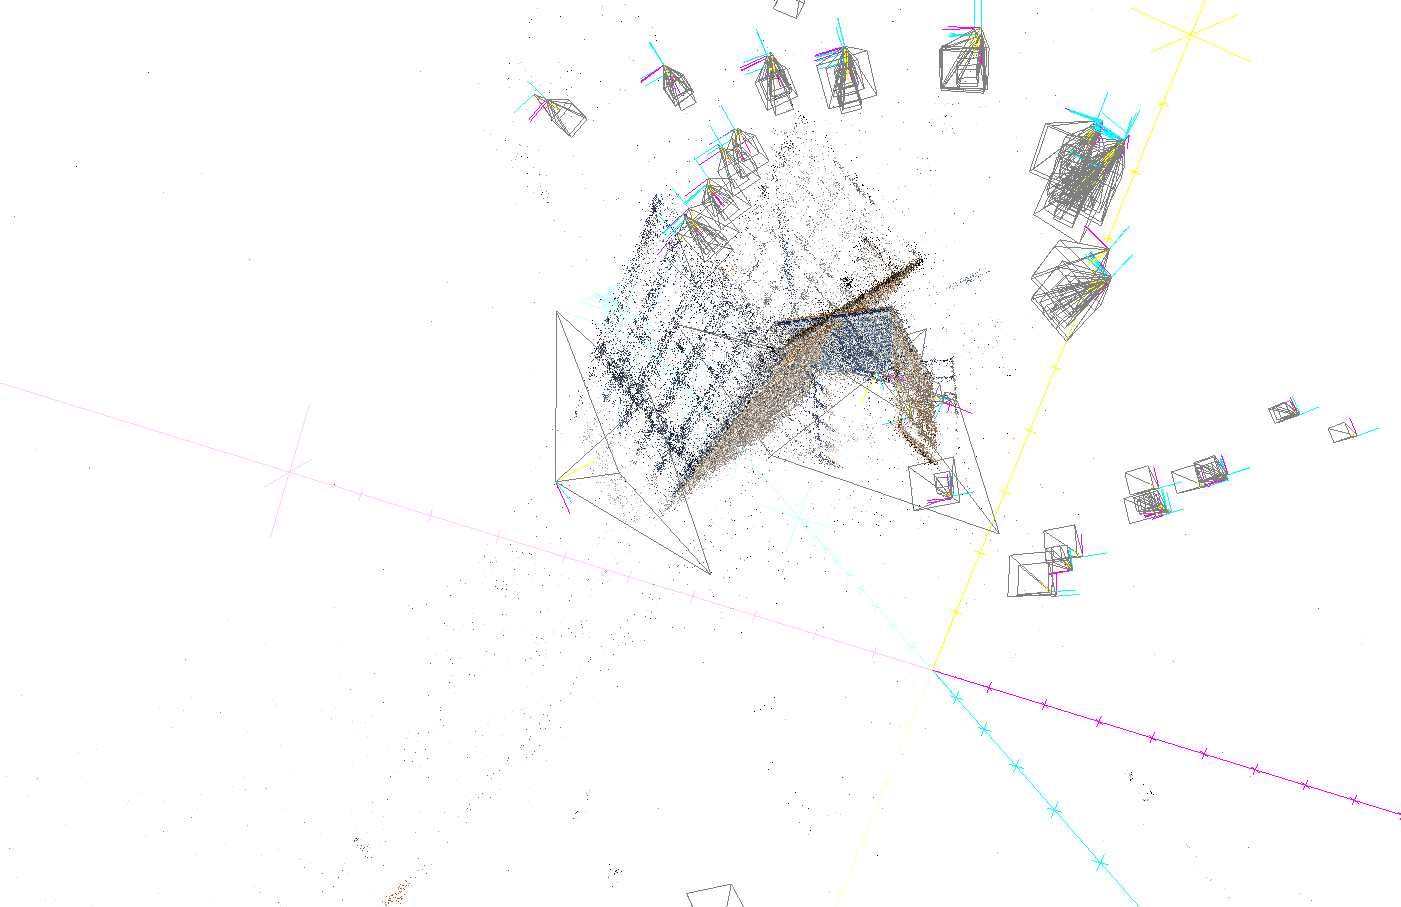
\includegraphics[height=0.3\textheight]{gfx/falscherekon1invert.png}
\caption[Fehlerhafte Rekonstruktion des AfE-Turms]{Fehlerhafte Rekonstruktion des AfE-Turms}
\label{gr:afeturmfehler}
\end{figure}
\FloatBarrier
Diese mangelhafte Rekonstruktion ist also auf eine fehlerhafte Paarbildung im Matchingverfahren zur\"uckzuf\"uhren, was gleichzeitig die Pr\"amisse des L\"osungsansatzes ist. 

\section{L\"osungsansatz und geplantes Vorgehen}
Da das Matchingverfahren im Moment f\"ur den Datensatz des AfE-Turms fehlschl\"agt, muss dieser Abschnitt der Software angepasst werden. Der hier vorgestellte Ansatz umfasst folglich die schon zuvor erw\"ahnten Anpassungen.\\
Durch die zus\"atzlichen Informationen die jedem Feature angeh\"oren, wird bei der Projektion eines Featuresets auf ein anderes die Definitionsmenge eingeschr\"ankt. Zu jedem Feature l\"asst sich \"uberpr\"ufen, welcher Region es angeh\"ort. Wohingegen zuvor nur eine Metrik als \"ahnlichkeitsma\ss  verwendet wurde, wird nun zuvor \"uberpr\"uft, ob ein korrespondierendes Feature-Paar auch den gleichen Regionen angeh\"ort, d.h. so k\"onnen keine fehlerhaften Feature-Paare mehr entstehen, dessen Elemente unterschiedlichen Regionen zugeteilt sind. Zwar nimmt mittels manueller Aufteilung der Fotografien das Verfahren vorab eine gewisse Zeit in Anspruch, die sich jedoch sp\"ater durch die gefilterte und somit reduzierte Feature-Menge in einem schnelleren und vor allem qualitativ besseren Rekonstruktionsablauf \"au\ss ern sollte.

\subsection{Bedeutung der Regionsabgrenzung}
Die MVE Pipeline besteht wie in den vorangegangenen Kapiteln beschrieben aus drei einzelnen Schritten, n\"amlich SfM, MVS und der Texturierung. Da sich SfM mit der Kalkulation der extrinsischen und intrinsischen Kameraparameter befasst und dazu die Regionierungsparameter bereits vorliegen m\"ussen, ist das Verfahren eindeutig davor einzuordnen. 

\begin{figure}[h]
\centering
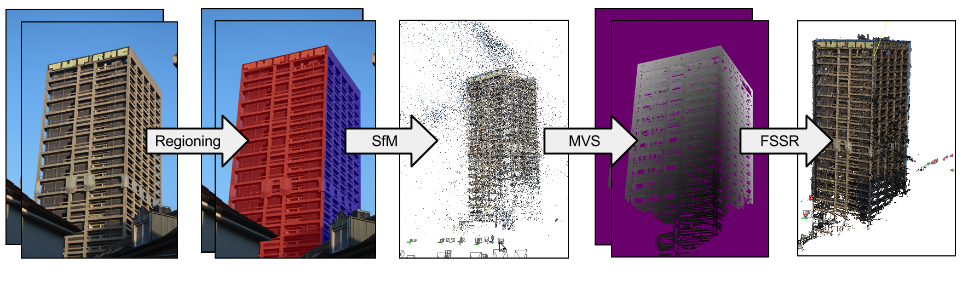
\includegraphics[width=0.9\textwidth]{gfx/pipeline.png}
\caption[MVE Pipeline]{MVE Pipeline}
\label{gr:pipeline}
\end{figure}
\FloatBarrier